% \documentclass[hyperref={pdfpagelabels=false},compress,table]{beamer} % 在Mac下无法编译
\documentclass[compress,table]{beamer} % 在Mac下使用
% package for font
\usepackage{fontspec}
\defaultfontfeatures{Mapping=tex-text}  %%如果没有它,会有一些 tex 特殊字符无法正常使用,比如连字符。
\usepackage{xunicode,xltxtra}
\usepackage[BoldFont,SlantFont,CJKnumber,CJKchecksingle]{xeCJK}  % \CJKnumber{12345}: 一万二千三百四十五
\usepackage{CJKfntef}  %%实现对汉字加点、下划线等。
\usepackage{pifont}  % \ding{}
% package for math
\usepackage{amsfonts}

% package for graphics
\usepackage[americaninductors,europeanresistors]{circuitikz}
\usepackage{tikz}
\usetikzlibrary{plotmarks}  % placements=positioning
\usepackage{graphicx}  % \includegraphics[]{}
\usepackage{subfigure}  %%图形或表格并排排列
% package for table
\usepackage{colortbl,dcolumn}  %% 彩色表格
\usepackage{multirow}
\usepackage{multicol}
\usepackage{booktabs}
% package for code
\usepackage{fancyvrb}
\usepackage{listings}

% \usepackage{animate}
% \usepackage{movie15}

%%%%%
% setting for beamer
\usetheme{default} % Madrid(常用), Copenhagen, AnnArbor, boxes(白色), Frankfurt,Berkeley
\useoutertheme[subsection=true]{miniframes} % 使用Berkeley时注释本行
\usecolortheme{sidebartab}
\usefonttheme{serif}  %%英文使用衬线字体
% \setbeamertemplate{background canvas}[vertical
% shading][bottom=white,top=structure.fg!7] %%背景色,上25%的蓝,过渡到下白。
\setbeamertemplate{theorems}[numbered]
\setbeamertemplate{navigation symbols}{}  %% 去掉页面下方默认的导航条
\setbeamercovered{transparent}  %设置 beamer 覆盖效果

% 设置标题title背景色
% \setbeamercolor{title}{fg=black, bg=lightgray!60!white}
\setbeamercolor{title}{fg=white, bg=black!70!white}

% 设置每页小LOGO
\pgfdeclareimage[width=1cm]{ouc}{figures/static/ouc.pdf}
\logo{\pgfuseimage{ouc}{\vspace{-20pt}}}

% setting for font
%%\setCJKmainfont{Adobe Kaiti Std}
\setCJKmainfont{SimSun} 
%% \setCJKmainfont{FangSong_GB2312} 
%% \setmainfont{Apple Garamond}  %%苹果字体没有SmallCaps
\setCJKmainfont{SimSun} 
%FUNNY%\setCJKmainfont{DFPShaoNvW5-GB}  %%华康少女文字W5(P)
%FUNNY%\setCJKmainfont{FZJingLeiS-R-GB}  %%方正静蕾体
%FUNNY%\setmainfont{Purisa}
%\setsansfont[Mapping=tex-text]{Adobe Song Std}
     %如果装了Adobe Acrobat,可在font.conf中配置Adobe字体的路径以使用其中文字体。
     %也可直接使用系统中的中文字体如SimSun、SimHei、微软雅黑等。
     %原来beamer用的字体是sans family;注意Mapping的大小写,不能写错。
     %设置字体时也可以直接用字体名,以下三种方式等同:
     %\setromanfont[BoldFont={黑体}]{宋体}
     %\setromanfont[BoldFont={SimHei}]{SimSun}
     %\setromanfont[BoldFont={"[simhei.ttf]"}]{"[simsun.ttc]"}
% setting for graphics
\graphicspath{{figures/}}  %%图片路径
\renewcommand\figurename{图}

% setting for pdf
\hypersetup{% pdfpagemode=FullScreen,%
            pdfauthor={Xiaodong Wang},%
            pdftitle={Title},%
            CJKbookmarks=true,%
            bookmarksnumbered=true,%
            bookmarksopen=false,%
            plainpages=false,%
            colorlinks=true,%
            citecolor=green,%
            filecolor=magenta,%
            linkcolor=blue,%red(default)
            urlcolor=cyan}

% setting for fontspec
\XeTeXlinebreaklocale "zh"  %%表示用中文的断行
\XeTeXlinebreakskip = 0pt plus 1pt minus 0.1pt  %%多一点调整的空间
%%%%%

% font setting by xeCJK
\setCJKfamilyfont{NSimSun}{NSimSun}
\newcommand{\song}{\CJKfamily{NSimSun}}
%%%\setCJKfamilyfont{AdobeSongStd}{Adobe Song Std}
%%%\newcommand{\AdobeSong}{\CJKfamily{AdobeSongStd}}
\setCJKfamilyfont{FangSong}{FangSong_GB2312}
\newcommand{\fang}{\CJKfamily{FangSong}}
%%%\setCJKfamilyfont{AdobeFangsongStd}{Adobe Fangsong Std}
%%%\newcommand{\AdobeFang}{\CJKfamily{AdobeFangsongStd}}
\setCJKfamilyfont{SimHei}{SimHei}
\newcommand{\hei}{\CJKfamily{SimHei}}
%%%\setCJKfamilyfont{AdobeHeitiStd}{Adobe Heiti Std}
%%%\newcommand{\AdobeHei}{\CJKfamily{AdobeHeitiStd}}
\setCJKfamilyfont{KaiTi}{KaiTi}
\newcommand{\kai}{\CJKfamily{KaiTi}}
%%%\setCJKfamilyfont{AdobeKaitiStd}{Adobe Kaiti Std}
\newcommand{\AdobeKai}{\CJKfamily{AdobeKaitiStd}}
\setCJKfamilyfont{LiSu}{LiSu}
\newcommand{\li}{\CJKfamily{LiSu}}
\setCJKfamilyfont{YouYuan}{YouYuan}
\newcommand{\you}{\CJKfamily{YouYuan}}
\setCJKfamilyfont{FZJingLei}{FZJingLeiS-R-GB}
\newcommand{\jinglei}{\CJKfamily{FZJingLei}}
\setCJKfamilyfont{MSYH}{Microsoft YaHei}
\newcommand{\msyh}{\CJKfamily{MSYH}}

% 自定义颜色
\def\Red{\color{red}}
\def\Green{\color{green}}
\def\Blue{\color{blue}}
\def\Mage{\color{magenta}}
\def\Cyan{\color{cyan}}
\def\Brown{\color{brown}}
\def\White{\color{white}}
\def\Black{\color{black}}

\lstnewenvironment{xmlCode}[1][]{% for Java
  \lstset{
    basicstyle=\tiny\ttfamily,%
    columns=flexible,%
    framexleftmargin=.7mm, %
    % frame=shadowbox,%
    % rulesepcolor=\color{cyan},%
     frame=single,%
    backgroundcolor=\color{white},%
    xleftmargin=4\fboxsep,%
    xrightmargin=4\fboxsep,%
    numbers=left,numberstyle=\tiny,%
    numberblanklines=false,numbersep=7pt,%
    language=xml, %
    }\lstset{#1}}{}

\lstnewenvironment{jspCode}[1][]{% for Java
  \lstset{
    basicstyle=\tiny\ttfamily,%
    columns=flexible,%
    framexleftmargin=.7mm, %
    % frame=shadowbox,%
    % rulesepcolor=\color{cyan},%
     frame=single,%
    backgroundcolor=\color{white},%
    xleftmargin=4\fboxsep,%
    xrightmargin=4\fboxsep,%
    numbers=left,numberstyle=\tiny,%
    numberblanklines=false,numbersep=7pt,%
    language=xml, %
    }\lstset{#1}}{}

\lstnewenvironment{javaCode}[1][]{% for Java
  \lstset{
    basicstyle=\tiny\ttfamily,%
    columns=flexible,%
    framexleftmargin=.7mm, %
    frame=shadowbox,%
    rulesepcolor=\color{cyan},%
    % frame=single,%
    backgroundcolor=\color{white},%
    xleftmargin=4\fboxsep,%
    xrightmargin=4\fboxsep,%
    numbers=left,numberstyle=\tiny,%
    numberblanklines=false,numbersep=7pt,%
    language=Java, %
    }\lstset{#1}}{}

\lstnewenvironment{shCode}[1][]{% for Java
  \lstset{
    basicstyle=\scriptsize\ttfamily,%
    columns=flexible,%
    framexleftmargin=.7mm, %
    frame=shadowbox,%
    rulesepcolor=\color{brown},%
    % frame=single,%
    backgroundcolor=\color{white},%
    xleftmargin=4\fboxsep,%
    xrightmargin=4\fboxsep,%
    numbers=left,numberstyle=\tiny,%
    numberblanklines=false,numbersep=7pt,%
    language=sh, %
    }\lstset{#1}}{}

\newcommand\ask[1]{\vskip 4bp \tikz \node[rectangle,rounded corners,minimum size=6mm,
  fill=white,]{\Cyan \includegraphics[height=1.5cm]{question} \Large \msyh #1};}

\newcommand\wxd[1]{\vskip 4bp \tikz \node[rectangle,minimum size=6mm,
  fill=blue!60!white,]{\White \ding{118} \msyh #1};}

\newcommand\xyy[1]{\vskip 2bp \tikz \node[rectangle,minimum size=3mm,
  fill=black!80!white,]{\White \msyh\scriptsize #1};}

\newcommand\cxf[1]{\vskip 4bp \tikz \node[rectangle,rounded corners,minimum size=6mm,
  fill=orange!60!white,]{\White \ding{42} \msyh #1};}

\newcommand\samp[1]{\vskip 2bp \tikz \node[rectangle,minimum size=3mm,
  fill=white!100!white,]{\Mage\msyh \small CODE \ding{231} \Black #1};\vskip -8bp}

\newcommand\zhyfly[1]{\tikz \node[rectangle,rounded corners,minimum size=6mm,ball color=red!25!blue,text=white,]{#1};}

\setbeamerfont{frametitle}{series=\msyh} % 修改Beamer标题字体

\makeatletter
\newcommand{\Extend}[5]{\ext@arrow 0099{\arrowfill@#1#2#3}{#4}{#5}}
\makeatother

%%%%%%%%%%%%%%%%%%%%%%%%%%%%%%%%%%%%%%%%%%%%%%%%
% \titlepage
\title[KevinW@OUC]{\hei {\huge Java EE企业应用系统设计}\\  
JSP}
\author[王晓东]{王晓东\\
  \href{mailto:wxd2870@163.com}{\footnotesize wxd2870@163.com}}
\institute[中国海洋大学]{\small 中国海洋大学}
\date{\today}
\titlegraphic{\vspace{-6em}
\includegraphics[height=6cm]{static/ouc.pdf}\vspace{-6em}}
%%%%%
\begin{document}
%% Delete this, if you do not want the table of contents to pop up at
%% the beginning of each subsection:
\AtBeginSection[]{                              % 在每个Section前都会加入的Frame
  \frame<handout:0>{
    \frametitle{\textbf{\hei 接下来…}}
    \tableofcontents[currentsection]
  }
}  %

\AtBeginSubsection[]                            % 在每个子段落之前
{
  \frame<handout:0>                             % handout:0 表示只在手稿中出现
  {
    \frametitle{\textit{\hei 接下来…}}\small
    \tableofcontents[current,currentsubsection] % 显示在目录中加亮的当前章节
  }
}
 \frame{\titlepage}

%%%%%%%%%%%%%%%%%%%%%%%%%%%%%%%%%%%%%%%%%%%%%%%%
\begin{frame}
\frametitle{参考书目}
\begin{enumerate}
\item 吕海东,张坤 编著,Java EE企业级应用开发实例教程,清华大学出版社,2010年8月
\end{enumerate}  
\end{frame}

% \begin{frame}
% \frametitle{本章学习目标}
% \begin{enumerate}
% \item 
% \end{enumerate}  
% \end{frame}

\section*{大纲}
\frame{\frametitle{大纲} \tableofcontents}

\section{JSP概述}

\begin{frame}
\frametitle{JSP基本概念}
\begin{itemize}
\item JSP,Java Server Page,即Java服务器页面。
\item JSP是Servlet的扩展。
\item 它将使用Java类编写动态Web组件转变为使用文本编写,降低了开发的难度。
\item JSP提供了一种自然的生成网页的方法。
\item 可以使用GUI工具来绘制JSP页面,而不是像Servlet写Java代码方法。
\item JSP文件的扩展名必须是 .jsp。
\end{itemize}
\end{frame}

\begin{frame}[fragile] % [fragile]参数使得能够插入代码
\frametitle{JSP的优点和缺点}
\wxd{优点}
\begin{itemize}
\item 编写动态Web网页更加容易;
\item 降低了开发难度;
\item 可以使用工具的拖拉方式生成JSP页面;
\item 纯文本文件。
\end{itemize}
\wxd{缺点}
\begin{itemize}
\item 非OO编程方式;
\item Java代码嵌入到HTML代码中,维护困难;
\item 不适合编写正常的业务处理应用程序。
\end{itemize}
\end{frame}

\begin{frame}[fragile] % [fragile]参数使得能够插入代码
\frametitle{JSP的执行过程} 
\begin{figure}
\centering
\includegraphics[width=0.8\textwidth]{jsp_01.png}
\end{figure}
\end{frame}

\begin{frame}[fragile] % [fragile]参数使得能够插入代码
\frametitle{JSP执行过程描述} 

\begin{enumerate}\kai
\item 客户使用浏览器通过HTTP请求JSP文件的URL地址,如:http://localhost:8080/web01/w/a.jsp;
\item Web服务器接收到请求,如果没有此地址,发出错误响应给浏览器;
\item Web服务器检查JSP文件和对应的Servlet版本的时间是否一致,如果一致则执行servlet的处理请求方法,类似于doGet或doPost,发送响应给浏览器;
\item 版本时间不一致,Web服务器调用转化系统,将JSP的文本代码转换为Servlet的Java代码;
\item 将Java代码编译为class文件;
\item 调用Servlet Class的响应方法。
\end{enumerate}
\end{frame}

\begin{frame}[fragile] % [fragile]参数使得能够插入代码
\frametitle{JSP页面的组成} 
一个JSP页面由{\hei HTML标记代码}和{\hei JSP元素}组成。HTML标记用于生成网页的静态部分,JSP元素用于生成动态内容部分。

\xyy{JSP元素}

\begin{description}
\item[JSP指令] 
\item[JSP动作] 
\item[JSP脚本] 
\item[JSP内置对象] 
\item[JSP扩展标记]
\end{description}
\end{frame}

\section{JSP指令}
\begin{frame}[fragile] % [fragile]参数使得能够插入代码
\frametitle{JSP指令} 
JSP指令指示一个JSP页面的属性和特征,JSP指令不会产生任何的输出到当前输出流中。

\wxd{JSP指令}
\begin{itemize}
\item page指令,用于定义JSP页面级的其他元素特征。
\item include指令,用于嵌入另一个文本文件的内容到本页面。
\item taglib指令,用于引入第三方JSP扩展标记类库。
\end{itemize}

\wxd{JSP指令的语法}
\begin{jspCode}
<%@ 指令名 属性名="值" 属性名="值" %>  
\end{jspCode}
\end{frame}

\begin{frame}[fragile] % [fragile]参数使得能够插入代码
\frametitle{Page指令 \ding{182}}
Page指令定义应用于整个页面的属性。

\xyy{语法}
\begin{jspCode}
<%@ page 属性名="属性值"  %>  
\end{jspCode}

\xyy{属性名和值}
\begin{itemize}
\item language="java",指定页面语言。
\item contentType="text/html; charset=gb2312",指定页面的内容类型,默认是text/html,可以指定显示的字符集,中文是gb2312 。
\item import="package, pageage",指定JSP页面使用的包和类,可以引用多个包,每个包用逗号分隔。
\end{itemize}
\end{frame}

\begin{frame}[fragile] % [fragile]参数使得能够插入代码
\frametitle{Page指令 \ding{183}}

\xyy{属性名和值}
\begin{itemize}
\item buffer="none | xkb",指定输出缓冲区容量,默认为8KB,buffer="9kb"。
\item errorPage="errorURL",指定错误页面地址,当页面出现异常时自动跳转到指定的错误页面。
\item isErrorPage="true|false",指定本页面是否是错误处理页面。
\item autoFlush="true | false",控制输出缓冲区是否自动清空,默认是true。
\end{itemize}
\end{frame}

\begin{frame}[fragile] % [fragile]参数使得能够插入代码
\frametitle{include指令}
include指令用于在当前网页中嵌入另一个网页,可以是JSP、HTML等。

\xyy{语法}
\begin{jspCode}
<%@ include file="url" %>
\end{jspCode}

\xyy{说明}
\begin{itemize}
\item file属性确定要嵌入的页面。
\item 嵌入页面的源代码被放置在此指令所在的位置。
\item 嵌入的用途是将一个复杂的页面分解为小的页面,然后使用include指令将他们再组装在一起。
\item {\Red 当修改被include的文件时,如果不修改主文件,则嵌入的内容不会改变。因此必须也修改主文件才能反映更新的嵌入文件。}
\end{itemize}
\end{frame}

\begin{frame}[fragile] % [fragile]参数使得能够插入代码
\frametitle{taglib指令} 
taglib指令用于引入扩展标签库,如JSTL、Struts、自定义标签库。

\xyy{语法}
\begin{jspCode}
<%@ taglib uri="/WEB-INF/tlds/struts-html.tld" prefix="html" %> 
<%@ taglib uri="http://java.sun.com/jsp/jstl/core" prefix="c" %>  
\end{jspCode}
\end{frame}

\section{JSP动作}

\begin{frame}[fragile,fragile] % [fragile]参数使得能够插入代码
\frametitle{JSP动作} 
JSP动作使用特定的符合XML格式的标记完成特定的任务
利用JSP动作可以完成动态的插入文件、重用JavaBean组件、把用户重定向到另外的页面、为Java插件生成HTML代码。

\wxd{JSP动作的语法}
\xyy{无嵌套封闭格式}
{\small\Blue
\begin{verbatim}
<jsp:动作名称 属性名="值" 属性名="值" 属性名="值"/>
\end{verbatim}}
\xyy{有嵌套封闭格式}
{\small\Blue
\begin{verbatim}
<jsp:动作名称 属性名="值" 属性名="值" 属性名="值">
  嵌入的其他动作
</jsp:动作名称>
\end{verbatim}}
\end{frame}

\begin{frame}[fragile] % [fragile]参数使得能够插入代码
\frametitle{JSP动作的类型} 
\begin{description}
\item[<jsp:include>] 嵌入其他页面输出内容动作;
\item[<jsp:forward>] 转发动作;
\item[<jsp:plugin>] 引入插件动作;
\item[<jsp:param>] 提供参数动作;
\item[<jsp:useBean>] 使用JavaBean动作;
\item[<jsp:setProperty>] 设置JavaBean属性动作;
\item[<jsp:getProperty>] 取得JavaBean属性动作。
\end{description}
\end{frame}

\subsection{include动作} 
\begin{frame}[fragile,fragile] % [fragile]参数使得能够插入代码
\frametitle{include动作} 

include动作用于嵌入其他页面的输出内容到此动作所在页面。

{\small\Blue
\begin{verbatim}
<jsp:include page="url" flush="true" />
\end{verbatim}

\begin{verbatim}
<jsp:include page="url" flush="true">
  <jsp:param name="参数名" value="参数值" />
</jsp:include>
\end{verbatim}
}
\begin{itemize}
\item page属性,指定嵌入页面的URL地址;
\item flush属性,指定是否在嵌入页面之前清空响应缓存区,默认为true;
\item jsp:param,为嵌入的页面传递参数,这些参数可以为动态、也可以为静态。
\end{itemize}
\end{frame}

\begin{frame}[fragile] % [fragile]参数使得能够插入代码
\frametitle{include指令和include动作的差异} 
\begin{itemize}
\item 其根本性不同在于他们被调用的时间。include指令在页面解析期间被嵌入;inlcude动作在请求的响应输出时被嵌入。
\item {\hei\Red 在实现文件包含上,因该尽可能的使用include动作。}
\item 而include指令存在的原因是其功能更加强大,执行速度稍快。
\end{itemize}

\begin{figure}
\centering
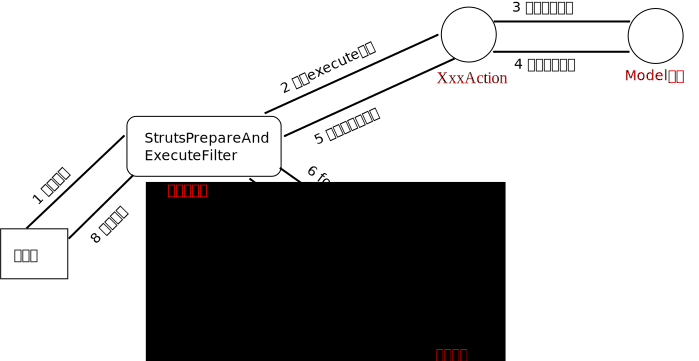
\includegraphics[width=0.6\textwidth]{fig01.pdf}
\end{figure}
\end{frame}

\subsection{useBean动作} 
\begin{frame}[fragile,fragile] % [fragile]参数使得能够插入代码
\frametitle{useBean动作} 
\begin{itemize}
\item 引用并调用JavaBean的方法和属性是JSP开发时必须面对的主要任务。
\item JSP为了简化JavaBean,提供了useBean动作标记,是的不必使用Java脚本代码,而使用标记方式取得JavaBean对象引用。
\end{itemize}

\wxd{useBean动作语法}
\begin{verbatim}
<jsp:useBean id="name" class="package.ClassName" 
  scope="page|request|session|application" />
\end{verbatim}

\begin{itemize}
\item id="name" 实例化变量名
\item scope="scope" 定义实例变量的生存周期范围
  \begin{itemize}
  \item page只在本页面中使用,默认值
  \item request在请求范围内有效
  \item session在会话范围内有效
  \item application在整个Web启动后有效
  \end{itemize}
\item class="package.ClassName" 指定JavaBean的类
\end{itemize}
\end{frame}

\begin{frame}[fragile] % [fragile]参数使得能够插入代码
\frametitle{useBean的执行过程} 
\begin{enumerate}\kai
\item 如果在指定范围内找到指定的对象,则得到此对象引用(即通过scope对象的getAttribute()方法)。
\item 如果没有找到指定的对象,则实例化一个class属性指定的对象(调用类的无参数构造方法)。
\item 对新建的对象执行嵌入的<jsp:setProperty />中指定的属性值,即调用JavaBean的setXXX方法,设置类的属性值。
\item 将对象保存到scope指定的范围的对象中,即调用内置对象的setAttribute(name,Object)方法,name是id指定的名称,object是类的对象。
\end{enumerate}
\end{frame}

\begin{frame}[fragile] % [fragile]参数使得能够插入代码
\frametitle{useBean动作示例} 
\xyy{JavaBean类User:User.java}
\begin{javaCode}
package com.city.oa.value;
import java.io.Serializable;  
public class User implements Serializable {
  private String id = null;
  private String password = null;
  private String name = null;
  private age = 0;

  public String getId() {
    return id;
  }
  public void setId(String id) {
    this.id = id;
  }
  ... ... // (other set/get methods.)
}
\end{javaCode}

\xyy{创建/取得指定的JavaBean对象,并保存在Request对象中}
\begin{jspCode}
<jsp:useBean id="user" class="com.city.oa.value.User" scope="request" \>
<%
  String name = user.getName();
  out.println(name);
%>
\end{jspCode}
\end{frame}

\begin{frame}[fragile] % [fragile]参数使得能够插入代码
\frametitle{使用useBean动作 VS. JSP脚本创建并取得对象引用} 
\begin{jspCode}
<% User user = new User(); %>
\end{jspCode}
{\centering VS.}
\begin{jspCode}
<jsp:useBean id="user" class="com.city.oa.value.User" scope="request" \>
\end{jspCode}
\begin{itemize}
\item 使用Java脚本创建的JavaBean,只能在本页面中使用,且每次都是创建新的JavaBean对象,不会保存在任何范围对象中。
\item useBean动作
  \begin{jspCode}
  <jsp:useBean id="user" class="com.city.oa.value.User" scope="request" \>    
  \end{jspCode}
  相当于如下Java脚本
  \begin{jspCode}
  <%
  User user = (User) request.getAttribute("user");
  if (user == null) {
    user = New User();
    request.setAttribute("user", user);
  }
  % >
  \end{jspCode}
\end{itemize}
\end{frame}

\subsection{setProperty动作} 
\begin{frame}[fragile] % [fragile]参数使得能够插入代码
\frametitle{setProperty动作} 
用于设定userBean动作取得的Bean对象的属性。相当于执行Bean对象的setXxx方法。

\begin{jspCode}
<jsp:setProperty name="beanId" property="*|name" param="参数名" value="value" />
\end{jspCode}

\begin{jspCode}
<jsp:useBean id="user" class="com.city.oa.value.User" scope="request" />
<jsp:setProperty name="user" property="name" value="吴明" >
\end{jspCode}
\end{frame}

\subsection{getProperty动作} 
\begin{frame}[fragile] % [fragile]参数使得能够插入代码
\frametitle{getProperty动作} 
用于取得Bean对象指定的属性值,转换为String类型,并显示在此动作所在的位置。

\begin{jspCode}
<jsp:getProperty name="beanId" property="属性名" />
\end{jspCode}

\begin{itemize}
\item name指定bean对象的名称,与useBean动作的id值对应;
\item property指定属性名,与JavaBean的getXxx方法对应。
\end{itemize}
\end{frame}

\subsection{forward动作} 
\begin{frame}[fragile] % [fragile]参数使得能够插入代码
\frametitle{forward动作} 
forward动作把请求转到另外的页面。

\xyy{无嵌入参数的转发动作}
\begin{jspCode}
<jsp:forward page="URL" />
\end{jspCode}

例如
\begin{jspCode}
<jsp:forward page="main.jsp" />  
\end{jspCode}

\xyy{有嵌入参数的转发动作}
\begin{jspCode}
<jsp:forward page="URL">
  <jsp:param name="参数名" value="值" />
  ... 
</jsp:forward>
\end{jspCode}
例如
\begin{jspCode}
<jsp:forward page="main.jsp">
  <jsp:param name="id" value="kevin" />
  <jsp:param name="password" value="1000" />
</jsp:forward>
\end{jspCode}
\end{frame}

\subsection{param动作} 
\begin{frame}[fragile] % [fragile]参数使得能够插入代码
\frametitle{param动作} 
param动作不能单独使用,需要嵌套在其他动作中,为其他动作提供参数,它可以嵌入到include、forward动作中为目标地址提供参数。例如:
\begin{jspCode}
<jsp:forward page="main.jsp">
  <jsp:param name="id" value="kevin" />
  <jsp:param name="password" value="1000" />
</jsp:forward>
\end{jspCode}
\end{frame}

\section{JSP脚本}

\begin{frame}[fragile,fragile,fragile,fragile,fragile] % [fragile]参数使得能够插入代码
\frametitle{JSP脚本类型}

\xyy{代码脚本}
\begin{jspCode}
<%
  int a=0; // 可以放置任何 Java 代码
%>
\end{jspCode}
\xyy{表达式脚本}
\begin{jspCode}
<%= a %> 用于输出 Java 表达式的值
\end{jspCode}
\xyy{声明脚本}
\begin{jspCode}
<%!
  int m=0; // 声明 JSP 类变量和方法
%>
\end{jspCode}
\xyy{注释脚本}
\begin{jspCode}
<%-- 注释 --%>
\end{jspCode}
\end{frame}

\begin{frame}[fragile] % [fragile]参数使得能够插入代码
\frametitle{代码脚本}
\begin{itemize}
\item 可以同时嵌入多个脚本代码段,但它们都表示在一个方法内,属于一个代码段,一个脚本内定义的变量,另一个脚本也可以使用。
\item 在代码脚本中定义的变量类似于Servlet的doGet方法中的局部变量,未初始化使用是非法的。
\end{itemize}

{\kai 例如,连接数据库的代码脚本片段如下:}
\begin{jspCode}
<%
  Connection cn = null;
  try {
    Class.forName("sun.jdbc.odbc.JdbcOdbc.Driver");
    cn  = DriverManager.getConnection("jdbc:odbc:cityoa");
    String sql = "select * from EMP";
    ... ...
  }
%>
\end{jspCode}
\end{frame}

\begin{frame}[fragile] % [fragile]参数使得能够插入代码
\frametitle{表达式脚本} 
注意:表达式后不能有分号;=号与<\%之间不能有空格,例如:
\begin{jspCode}
<%= rs.getString("NAME") %>
\end{jspCode}
\end{frame}

\begin{frame}[fragile] % [fragile]参数使得能够插入代码
\frametitle{声明脚本} 
用于声明JSP页面的类变量和方法。

由于JSP在运行时会转换为Servlet类,声明的脚本部分会成为类中定义的一部分。
例如:
\begin{jspCode}
<%!
  int num = 0;
  public void addNum() {
    num++;
  }
%>
\end{jspCode}
如下声明脚本有错误:
\begin{jspCode}
<%!
  int num = 0;
  num++; // 错误,声明脚本中不能直接有非声明代码
%>  
\end{jspCode}
\end{frame}

\begin{frame}[fragile] % [fragile]参数使得能够插入代码
\frametitle{注释脚本} 
在JSP页面中可以使用HTML注释:
\begin{jspCode}
<!-- HTML Comment -->
\end{jspCode}
{\kai\Red 但是,使用HTML注释不安全,因为HTML注释随着JSP生成的HTML响应下载到客户端浏览器,客户可以看到。}

JSP注释是服务器端技术,在服务器端处理,不会发送到客户端,比较安全。
\begin{jspCode}
<%-- JSP Comment --%>  
\end{jspCode}
\end{frame}

\section{JSP内置对象} 

\begin{frame}[fragile] % [fragile]参数使得能够插入代码
\frametitle{JSP内置对象} 

JSP作为Web组件,为和Web容器以及其他Web组件进行通信和协作,提供了内置的与HTTP请求和响应相
关的对象,这些对象不需要定义和引用,在JSP代码脚本和表达式脚本中可以直接使用。
\begin{itemize}\kai
\item request 请求对象
\item response 响应对象
\item session 会话对象
\item application 应用服务器对象
\item page JSP本身页面类对象
\item pageContext 页面级环境变量,作为页面级容器
\item out 输出对象
\item exception 异常对象
\item config 配置对象,用于读取web.xml配置信息
\end{itemize}
\end{frame}

\begin{frame}[fragile] % [fragile]参数使得能够插入代码
\frametitle{请求对象request} 
request与Servlet中传递的请求对象相同,类型为javax.servlet.http.HttpServletRequest。
\xyy{常见方法}
\begin{itemize}
\item Object getAttribute(String name) 返回指定属性的属性值
\item Enumeration getAttrbuteNames() 返回所有可用属性名的枚举
\item String getCharacterEncoding() 返回字符编码的方式
\item String getParameter(String name) 返回指定参数的参数值
\item ...
\end{itemize}
\end{frame}

\begin{frame}[fragile] % [fragile]参数使得能够插入代码
\frametitle{响应对象response} 
JSP页面使用文本方式实现HTTP响应,所以JSP内部response对象没有像Servlet中响应对象使用那么频繁,在JSP中实现响应,直接将响应内容写在JSP页面就可以,不需要使用响应对象取得PrintWriter对象,再进行响应输出。

响应对象类型为javax.servlet.http.HttpServletResponse,JSP使用不是很多。
\xyy{常见方法}
\begin{itemize}
\item String getCharacterEncoding() 返回响应用的是何种编码
\item ...
\end{itemize}
\end{frame}

\begin{frame}[fragile] % [fragile]参数使得能够插入代码
\frametitle{会话对象session} 

JSP的session对象对应Servlet中的javax.servlet.http.HttpSession。

JSP页面使用page指令
\begin{jspCode}
<%@ page session="true | false" %> 
\end{jspCode}
指示此JSP页面是否可以使用session内置对象。

\xyy{常见方法}
\begin{itemize}\kai\small
\item long getCreationTime() 返回session创建时间
\item public String getId() 返回session创建是JSP引擎为它设置的唯一ID号
\item long getLastAccessdTime() 返回此session中客户端最近一次请求的时间
\item int getMaxInactiveInterval() 返回两起请求间隔多长时间此session被取消
\item String[] getValueNames() 返回一个包含此session中所有可用属性的数组
\item void invalidate() 取消session,使其不可用
\end{itemize}
\end{frame}

\begin{frame}[fragile] % [fragile]参数使得能够插入代码
\frametitle{服务器环境对象application} 
\begin{itemize}
\item appliation对应Servlet中的javax.servlet.ServletContext对象实例。
\item 每个Web站点只有一个application对象。
\item application对象是一个Map类型的容器。
\item application作为Web级的容器,保存整个Web应用个Web组件之间需要共享的数据,application可以保存整个请求用户都可以访问的共享信息。
\item 在保存信息到application时,要注意多用户同时写的线程同步问题。
\end{itemize}

\xyy{常用方法}
\begin{itemize}
\item 存入数据方法 void setAttribute(String name,Object object);
\item 读取数据的方法 Object getAttribute(String name);
\item 删除数据的方法 void removeAttribute(String name);
\end{itemize}
\end{frame}

\begin{frame}[fragile] % [fragile]参数使得能够插入代码
\frametitle{页面对象page} 

page对象就是指向当前JSP页面本身,有点像类中的this指针,它是java.lang.Object的实例,在JSP编程中应用较少。

\xyy{常用方法}
\begin{itemize}
\item int hashCode() 返回此Object的hash码
\end{itemize}
\end{frame}

\begin{frame}[fragile] % [fragile]参数使得能够插入代码
\frametitle{页面环境对象pageContext} 
略。
\end{frame}

\begin{frame}[fragile] % [fragile]参数使得能够插入代码
\frametitle{输出对象out} 

out内置对象即JSP页面向浏览器发出响应流PrintWriter的实例对象。但JSP页面可以直接放入响应文本,因此JSP页面基本不使用out进行文本响应。

一般情况下使用
\begin{jspCode}
<%= %>  
\end{jspCode}
来代替使用out对象。
\end{frame}

\begin{frame}[fragile] % [fragile]参数使得能够插入代码
\frametitle{异常对象exception} 

JSP内置对象exception对应Java中的java.lang.Throwable接口对象。它自动封装JSP页面中出现的异
常。异常对象只有在错误页面中可以使用,即使用page指令的属性{\Blue isErrorPage="true"}声明的页面。

\xyy{exception01.jsp}
\begin{jspCode}
<%@ page language="java" contentType="text/html; charset=utf-8" 
    errorPage="error.jsp" import="java.util.*" pageEncoding="utf-8" %>
<html>
<head>
<meta http-equiv="Content-Type" content="text/html; charset=utf-8">
<title>Test Exception</title>
</head>
<body>
<%
	int s = 0;
	int t = 0; 
	int p = s / t; // 出现异常的语句
%>
</body>
</html>  
\end{jspCode}
\end{frame}

\begin{frame}[fragile] % [fragile]参数使得能够插入代码
\frametitle{异常对象exception} 
\xyy{error.jsp}
\begin{jspCode}
<%@ page language="java" contentType="text/html; charset=utf-8" isErrorPage="true"
    pageEncoding="utf-8"%>
<html>
<head>
<meta http-equiv="Content-Type" content="text/html; charset=utf-8">
<title>Error Page</title>
</head>
<body>
<h1>异常显示信息</h1>
错误原因:<%= exception.getMessage() %>
</body>
</html>  
\end{jspCode}

{\kai\Red 使用errorPage方式实现的页面跳转,使用的是转发方式,而不是重定向模式。}
\end{frame}

\begin{frame}[fragile] % [fragile]参数使得能够插入代码
\frametitle{配置对象config} 

congfig对象提供对JSP页面的javax.servlet.ServletConfig对象的访问。例如:

\begin{jspCode}
<%= config.getInitParameter("driverName") %>
\end{jspCode}
\end{frame}

%%%%%%%%%%%%%%%%%%%%%%%%%%
\begin{frame}[fragile] % [fragile]参数使得能够插入代码
\frametitle{} 

\end{frame}
%%%%%%%%%%%%%%%%%%%%%%%%%%
%% \begin{figure}
%% \centering
%% 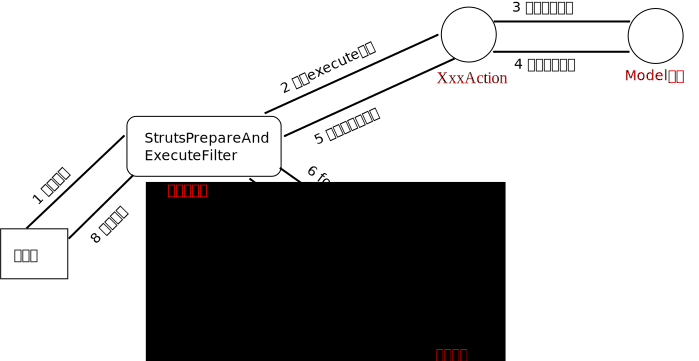
\includegraphics[width=0.6\textwidth]{fig01.png}
%% \end{figure}
% TKS %%%%%%%%%%%%%%%%%%%%%%%%%%%%%%%%%%%%%%%%%%%%%%
\begin{frame}
\centering
{\Huge \textcolor{blue}{THE END}} \\
\vspace{5mm}
{\Large wxd2870@163.com} \\
\end{frame}
%%%%%%%%%%%%%%%%%%%%%%%%%%%%%%%%%%%%%%%%%%%%%%%%%%
\end{document}

%% Refs
%% Session and Cookie http://my.oschina.net/dingyuan963/blog/9194